\documentclass[11pt,a4paper]{report}
\usepackage[textwidth=37em,vmargin=30mm]{geometry}
\usepackage{calc,xunicode,amsmath,amssymb,paralist,enumitem,tabu,booktabs,datetime2,xeCJK,xeCJKfntef,listings}
\usepackage{tocloft,fancyhdr,tcolorbox,xcolor,graphicx,eso-pic,xltxtra,xelatexemoji}

\newcommand{\envyear}[0]{2025}
\newcommand{\envdatestr}[0]{2025-09-21}
\newcommand{\envfinaldir}[0]{webdb/2025/20250921/final}

\usepackage[hidelinks]{hyperref}
\hypersetup{
    colorlinks=false,
    pdfpagemode=FullScreen,
    pdftitle={Web Digest - \envdatestr}
}

\setlength{\cftbeforechapskip}{10pt}
\renewcommand{\cftchapfont}{\rmfamily\bfseries\large\raggedright}
\setlength{\cftbeforesecskip}{2pt}
\renewcommand{\cftsecfont}{\sffamily\small\raggedright}

\setdefaultleftmargin{2em}{2em}{1em}{1em}{1em}{1em}

\usepackage{xeCJK,xeCJKfntef}
\xeCJKsetup{PunctStyle=plain,RubberPunctSkip=false,CJKglue=\strut\hskip 0pt plus 0.1em minus 0.05em,CJKecglue=\strut\hskip 0.22em plus 0.2em}
\XeTeXlinebreaklocale "zh"
\XeTeXlinebreakskip = 0pt


\setmainfont{Brygada 1918}
\setromanfont{Brygada 1918}
\setsansfont{IBM Plex Sans}
\setmonofont{JetBrains Mono NL}
\setCJKmainfont{Noto Serif CJK SC}
\setCJKromanfont{Noto Serif CJK SC}
\setCJKsansfont{Noto Sans CJK SC}
\setCJKmonofont{Noto Sans CJK SC}

\setlength{\parindent}{0pt}
\setlength{\parskip}{8pt}
\linespread{1.15}

\lstset{
	basicstyle=\ttfamily\footnotesize,
	numbersep=5pt,
	backgroundcolor=\color{black!5},
	showspaces=false,
	showstringspaces=false,
	showtabs=false,
	tabsize=2,
	captionpos=b,
	breaklines=true,
	breakatwhitespace=true,
	breakautoindent=true,
	linewidth=\textwidth
}






\newcommand{\coverpic}[2]{
    % argv: itemurl, authorname
    Cover photo by #2~~(\href{#1}{#1})
}
\newcommand{\makeheader}[0]{
    \begin{titlepage}
        % \newgeometry{hmargin=15mm,tmargin=21mm,bmargin=12mm}
        \begin{center}
            
            \rmfamily\scshape
            \fontspec{BaskervilleF}
            \fontspec{Old Standard}
            \fontsize{59pt}{70pt}\selectfont
            WEB\hfill DIGEST
            
            \vfill
            % \vskip 30pt
            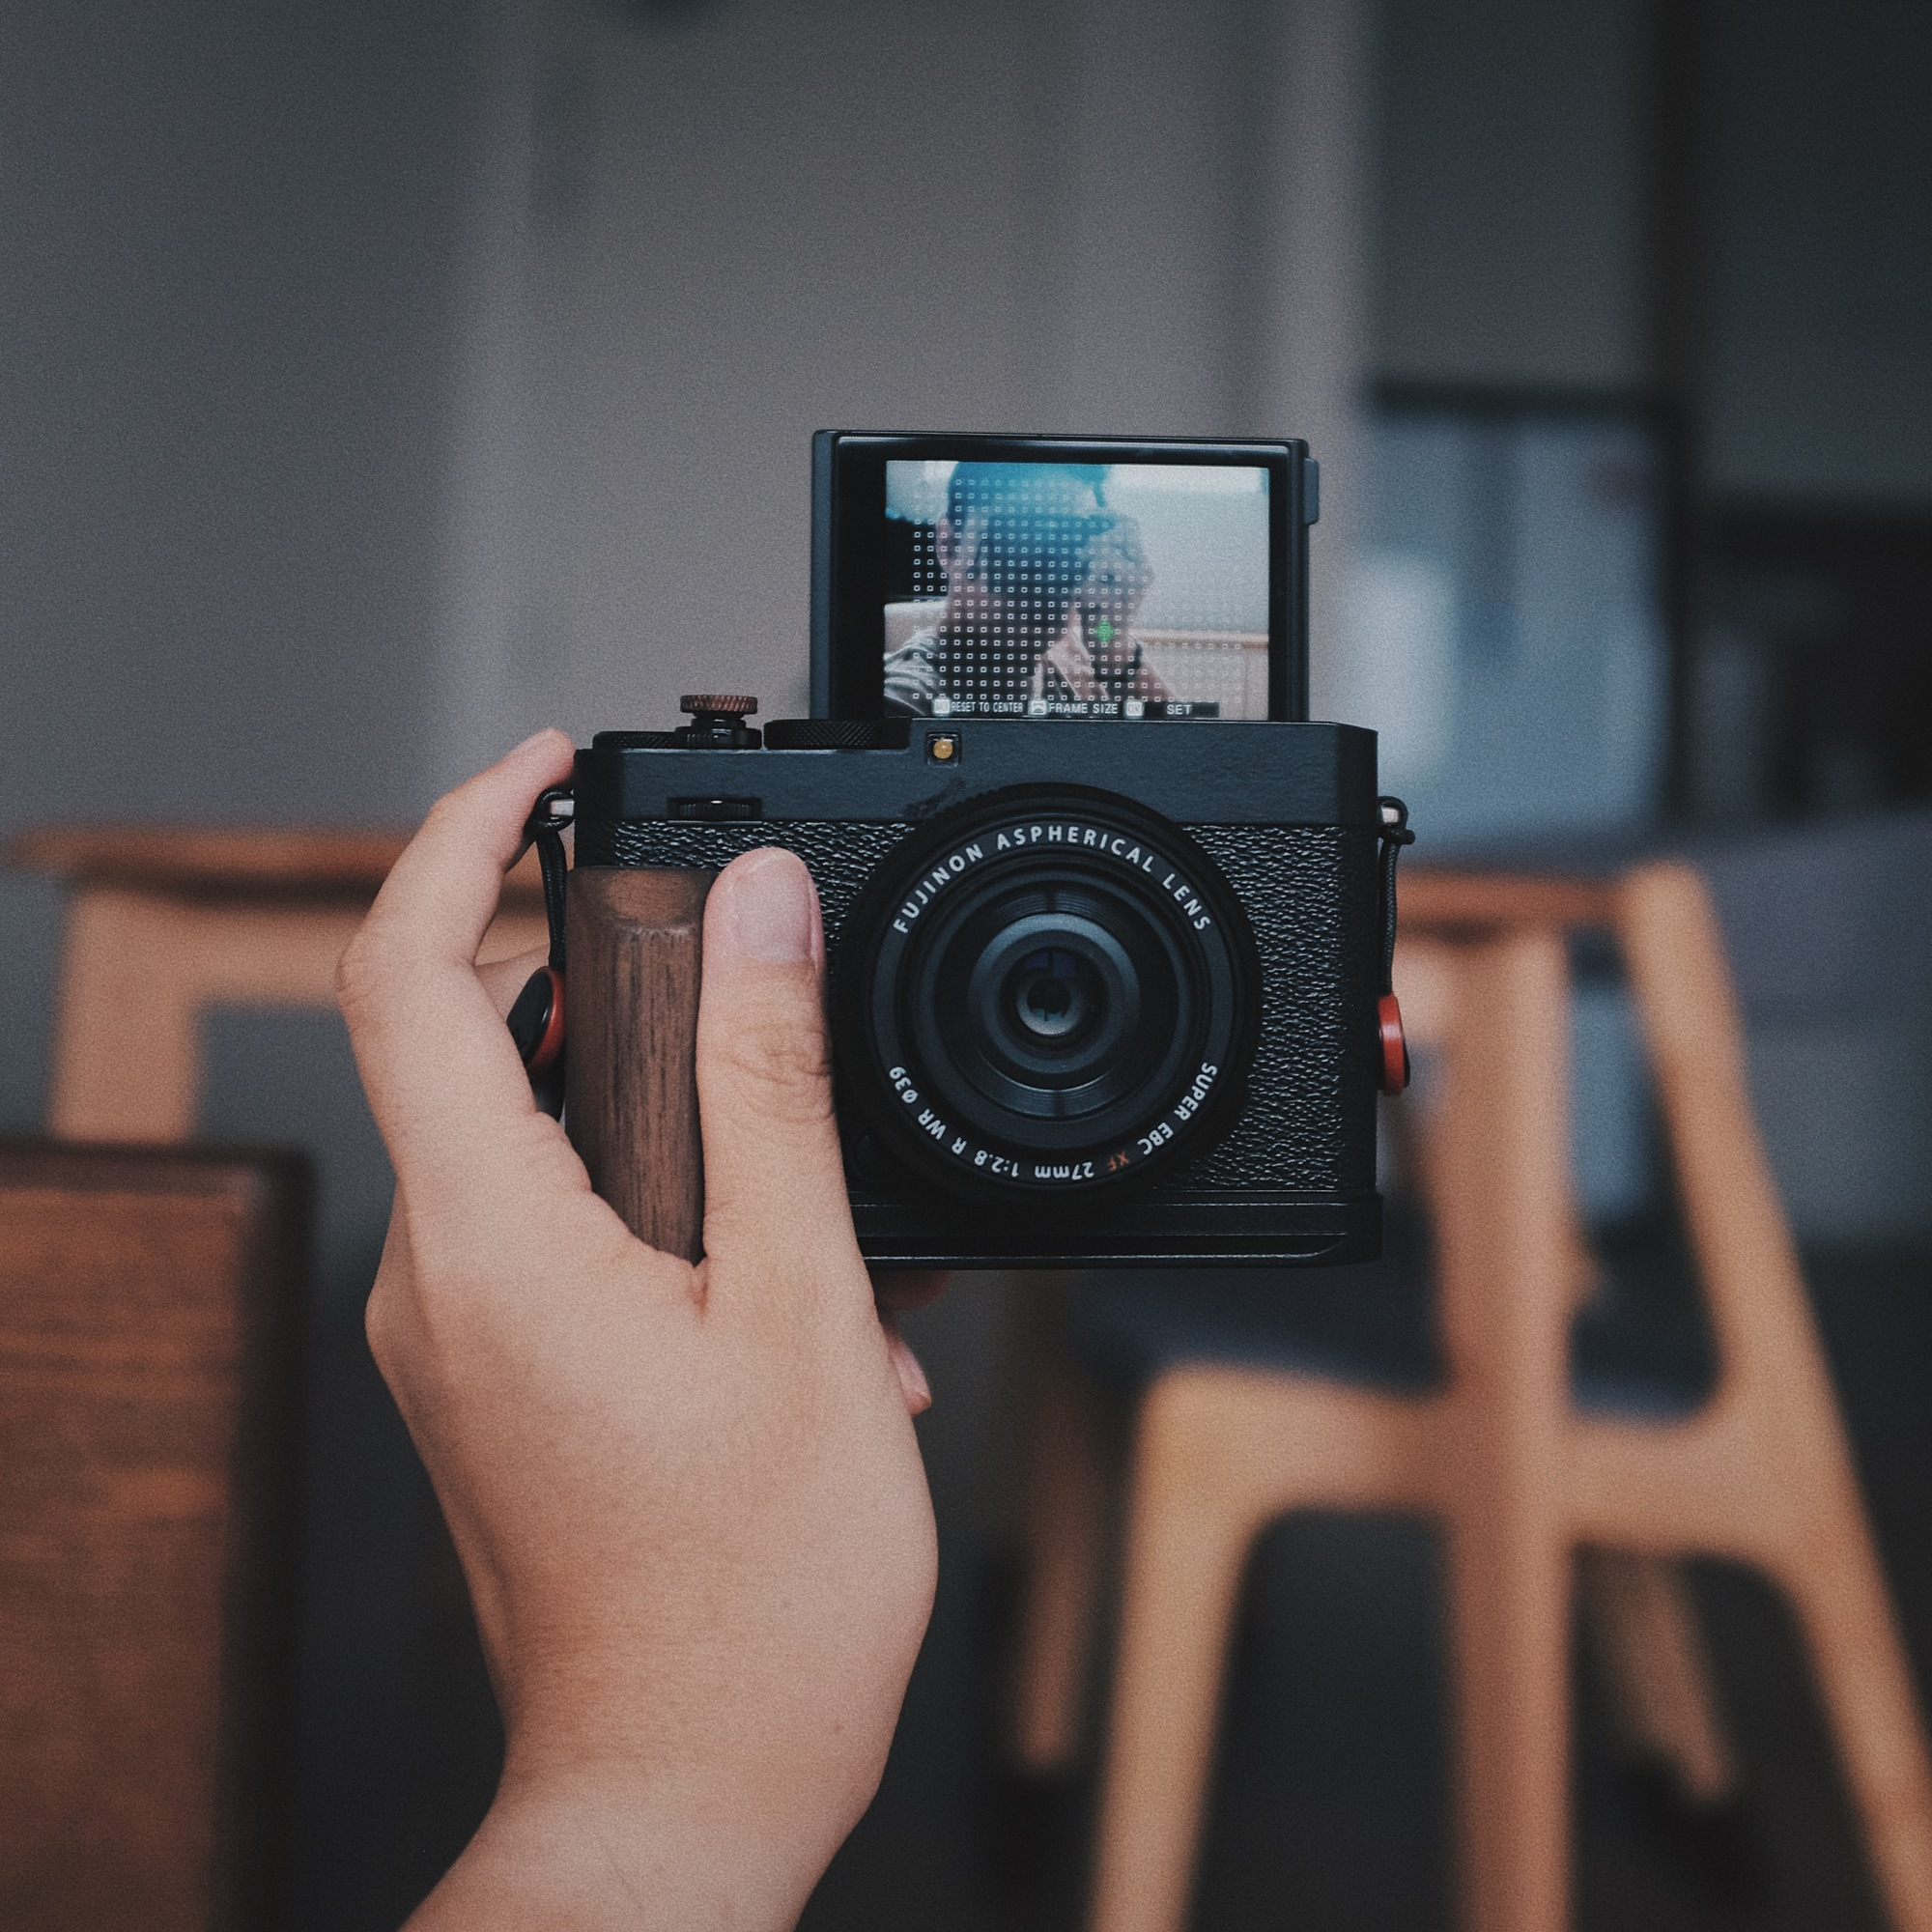
\includegraphics[width=\linewidth]{\envfinaldir/coverpic-prod.jpg}\par
            % \vskip 30pt
            \vfill

            \normalsize\rmfamily\scshape
            \copyright{} The Web Digest Project \hfill\large \envdatestr
        \end{center}
    \end{titlepage}
    % \restoregeometry
}
\newcommand{\simplehref}[1]{%
    \textcolor{blue!80!green}{\href{#1}{#1}}%
}
\renewcommand{\contentsname}{\center\Huge\sffamily\bfseries Contents\par\vskip 20pt}
\newcounter{ipartcounter}
\setcounter{ipartcounter}{0}
\newcommand{\ipart}[1]{
    % \vskip 20pt
    \clearpage
    \stepcounter{ipartcounter}
    \phantomsection
    \addcontentsline{toc}{chapter}{#1}
    % \begin{center}
    %     \Huge
    %     \sffamily\bfseries
    %     #1
    % \end{center}
    % \vskip 20pt plus 7pt
}
\newcounter{ichaptercounter}
\setcounter{ichaptercounter}{0}
\newcommand{\ichapter}[1]{
    % \vskip 20pt
    \clearpage
    \stepcounter{ichaptercounter}
    \phantomsection
    \addcontentsline{toc}{section}{\numberline{\arabic{ichaptercounter}}#1}
    \begin{center}
        \Huge
        \sffamily\bfseries
        #1
    \end{center}
    \vskip 20pt plus 7pt
}
\newcommand{\entrytitlefont}[1]{\subsection*{\raggedright\Large\sffamily\bfseries#1}}
\newcommand{\entryitemGeneric}[2]{
    % argv: title, url
    \parbox{\linewidth}{
        \entrytitlefont{#1}\par\vskip 5pt
        \footnotesize\ttfamily\mdseries
        \simplehref{#2}
    }\vskip 11pt plus 11pt minus 1pt
}
\newcommand{\entryitemGithub}[3]{
    % argv: title, url, desc
    \parbox{\linewidth}{
        \entrytitlefont{#1}\par\vskip 5pt
        \footnotesize\ttfamily\mdseries
        \simplehref{#2}\par\vskip 5pt
        \small\rmfamily\mdseries#3
    }\vskip 11pt plus 11pt minus 1pt
}
\newcommand{\entryitemAp}[3]{
    % argv: title, url, desc
    \parbox{\linewidth}{
        \entrytitlefont{#1}\par\vskip 5pt
        \footnotesize\ttfamily\mdseries
        \simplehref{#2}\par\vskip 5pt
        \small\rmfamily\mdseries#3
    }\vskip 11pt plus 11pt minus 1pt
}
\newcommand{\entryitemHackernews}[3]{
    % argv: title, hnurl, rawurl
    % \parbox{\linewidth}{
    %     \entrytitlefont{#1}\par\vskip 5pt
    %     \footnotesize\ttfamily\mdseries
    %     \simplehref{#3}\par
    %     \textcolor{black!50}{\href{#2}{#2}}
    % }\vskip 11pt plus 11pt minus 1pt
    \begin{minipage}{\linewidth}
            \entrytitlefont{#1}\par\vskip 5pt
            \footnotesize\ttfamily\mdseries
            \simplehref{#3}\par
            \textcolor{black!50}{\href{#2}{#2}}
    \end{minipage}\par\vskip 11pt plus 11pt minus 1pt
}







\begin{document}

\makeheader

\tableofcontents\clearpage




\ipart{Developers}
\ichapter{Hacker News}
\entryitemTwoLinks{\$2 WeAct Display FS adds a 0.96-inch USB information display to your computer}{https://news.ycombinator.com/item?id=45317527}{https://www.cnx-software.com/2025/09/18/2-weact-display-fs-adds-a-0-96-inch-usb-information-display-to-your-computer/}

\entryitemTwoLinks{The LLM Lobotomy?}{https://news.ycombinator.com/item?id=45315746}{https://learn.microsoft.com/en-us/answers/questions/5561465/the-llm-lobotomy}

\entryitemTwoLinks{Designing NotebookLM}{https://news.ycombinator.com/item?id=45315312}{https://jasonspielman.com/notebooklm}

\entryitemTwoLinks{Microsoft memo advises H1B employees to return immediately if currently abroad}{https://news.ycombinator.com/item?id=45314906}{https://x.com/onestpress/status/1969374699038675364}

\entryitemTwoLinks{Ultrasonic Chef's Knife}{https://news.ycombinator.com/item?id=45314592}{https://seattleultrasonics.com/}

\entryitemTwoLinks{Are touchscreens in cars dangerous?}{https://news.ycombinator.com/item?id=45314432}{https://www.economist.com/science-and-technology/2025/09/19/are-touchscreens-in-cars-dangerous}

\entryitemTwoLinks{Britain jumps into bed with Palantir in £1.5B defense pact}{https://news.ycombinator.com/item?id=45313793}{https://www.theregister.com/2025/09/20/uk\_palantir\_defense\_pact/}

\entryitemTwoLinks{Is Zig's new writer unsafe?}{https://news.ycombinator.com/item?id=45313597}{https://www.openmymind.net/Is-Zigs-New-Io-Unsafe/}

\entryitemTwoLinks{Cormac McCarthy's tips on how to write a science paper (2019) [pdf]}{https://news.ycombinator.com/item?id=45313557}{https://gwern.net/doc/science/2019-savage.pdf}

\entryitemTwoLinks{Microsoft has urged its employees on H-1B and H-4 visas to return immediately}{https://news.ycombinator.com/item?id=45312877}{https://timesofindia.indiatimes.com/technology/tech-news/microsoft-has-a-24-hour-deadline-warning-for-indian-and-other-foreign-employees-after-h1-b-visa-fees-hike-to-100000-strongly-recommend-h1b-visa-holders-/articleshow/124010245.cms}

\entryitemTwoLinks{Git: Introduce Rust and announce it will become mandatory in the build system}{https://news.ycombinator.com/item?id=45312696}{https://lore.kernel.org/git/20250904-b4-pks-rust-breaking-change-v1-0-3af1d25e0be9@pks.im/}

\entryitemTwoLinks{Images over DNS}{https://news.ycombinator.com/item?id=45312515}{https://dgl.cx/2025/09/images-over-dns}

\entryitemTwoLinks{FLX1s phone is launched}{https://news.ycombinator.com/item?id=45312326}{https://furilabs.com/flx1s-is-launched/}

\entryitemTwoLinks{IG Nobel Prize Winners 2025}{https://news.ycombinator.com/item?id=45312228}{https://improbable.com/ig/winners/}

\entryitemTwoLinks{If you are good at code review, you will be good at using AI agents}{https://news.ycombinator.com/item?id=45310529}{https://www.seangoedecke.com/ai-agents-and-code-review/}

\entryitemTwoLinks{Things managers do that leaders never would}{https://news.ycombinator.com/item?id=45309512}{https://simonsinek.com/stories/5-things-managers-do-that-leaders-never-would-according-to-simon/}

\entryitemTwoLinks{Trumpcard (Official US Government Website)}{https://news.ycombinator.com/item?id=45308778}{https://trumpcard.gov/}

\entryitemTwoLinks{H1Bs will start costing \$100k/yr}{https://news.ycombinator.com/item?id=45308628}{https://www.boundless.com/blog/trump-administration-to-propose-new-100000-fee-for-h-1b-visa-applications/}

\entryitemTwoLinks{Disney+ cancellation page crashes as customers rush to quit}{https://news.ycombinator.com/item?id=45308558}{https://creators.yahoo.com/lifestyle/story/disney-cancellation-page-crashes-as-customers-rush-to-quit-after-kimmel-suspension-033512277.html}

\entryitemTwoLinks{Did you read the quarter-million-line license for your Slack app?}{https://news.ycombinator.com/item?id=45308503}{https://mastodon.mit.edu/@Eggfreckles/114825126857396420}\ichapter{Phoronix}
\entryitemGeneric{\hskip 0pt{}Git Developers Debate Making Rust Mandatory}{https://www.phoronix.com/news/Git-Weighs-Mandatory-Rust}

\entryitemGeneric{\hskip 0pt{}Ad-Free Viewing By Showing Your Support During The Phoronix Oktoberfest / Autumn Sale}{https://www.phoronix.com/news/Phoronix-Fall-Promotion-2025}

\entryitemGeneric{\hskip 0pt{}Debian's APT Gaining Built-In History Command}{https://www.phoronix.com/news/Debian-APT-History-Command}

\entryitemGeneric{\hskip 0pt{}AMD ISP4 Driver Still Pending Review For The Linux Kernel}{https://www.phoronix.com/news/AMD-ISP4-Driver-Pending-Review}

\entryitemGeneric{\hskip 0pt{}DKMS Packages For Bcachefs Are Now Available On Debian \& Ubuntu}{https://www.phoronix.com/news/Bcachefs-Debian-Ubuntu-DKMS}

\entryitemGeneric{\hskip 0pt{}KDE Plasma 6.5 Preps Yet More Wayland Fixes \& Improvements}{https://www.phoronix.com/news/Plasma-6.5-More-Wayland-Work}

\entryitemGeneric{\hskip 0pt{}Linux 6.17 File-System Benchmarks, Including OpenZFS \& Bcachefs}{https://www.phoronix.com/review/linux-617-filesystems}

\entryitemGeneric{\hskip 0pt{}Mesa Adds Contributor Guidelines - Will Allow AI Generated Code If Author Understands It}{https://www.phoronix.com/news/Mesa-Contributor-Guidelines}

\entryitemGeneric{\hskip 0pt{}Ubuntu Now Has Daily Dangerous Desktop Images}{https://www.phoronix.com/news/Ubuntu-Daily-Dangerous}


\ipart{Developers~~~~(zh-Hans)}
\ichapter{Solidot}
\entryitemGeneric{\hskip 0pt{}小米将远程修复其 11 万辆 SU7 的辅助驾驶系统缺陷}{https://www.solidot.org/story?sid=82370}

\entryitemGeneric{\hskip 0pt{}美国要求 H-1B 签证申请支付 10 万美元}{https://www.solidot.org/story?sid=82369}

\entryitemGeneric{\hskip 0pt{}华为和浙江大学发布 DeepSeek-R1-Safe}{https://www.solidot.org/story?sid=82368}

\entryitemGeneric{\hskip 0pt{}狗能根据玩具功能对其进行分类}{https://www.solidot.org/story?sid=82367}

\entryitemGeneric{\hskip 0pt{}诺格的补给飞船解决了软件问题成功抵达国际空间站}{https://www.solidot.org/story?sid=82366}

\entryitemGeneric{\hskip 0pt{}汽车行业制造了远超需求的汽车}{https://www.solidot.org/story?sid=82363}

\entryitemGeneric{\hskip 0pt{}Steam 将从 2026 年起不再支持 32 位 Windows 操作系统}{https://www.solidot.org/story?sid=82362}

\entryitemGeneric{\hskip 0pt{}新材料拉伸率达到 46 倍且能自我修复}{https://www.solidot.org/story?sid=82361}

\entryitemGeneric{\hskip 0pt{}2025 年度搞笑诺贝尔奖宣布}{https://www.solidot.org/story?sid=82360}

\entryitemGeneric{\hskip 0pt{}Google 为美国用户的 Chrome 浏览器集成 Gemini AI 功能}{https://www.solidot.org/story?sid=82359}

\entryitemGeneric{\hskip 0pt{}三星推送软件更新为冰箱加入广告}{https://www.solidot.org/story?sid=82358}

\entryitemGeneric{\hskip 0pt{}斑胸草雀具有语义理解能力}{https://www.solidot.org/story?sid=82357}

\entryitemGeneric{\hskip 0pt{}英伟达向英特尔投资 50 亿美元}{https://www.solidot.org/story?sid=82356}

\entryitemGeneric{\hskip 0pt{}研究发现珊瑚无法在一个更温暖的世界里生存下来}{https://www.solidot.org/story?sid=82355}

\entryitemGeneric{\hskip 0pt{}DeepSeek 发表 R1 模型论文,称训练成本仅 29.4 万美元}{https://www.solidot.org/story?sid=82354}

\entryitemGeneric{\hskip 0pt{}全球变暖致日本危险性高温日增加 22 天}{https://www.solidot.org/story?sid=82353}

\entryitemGeneric{\hskip 0pt{}NASA 确认了逾六千颗系外行星}{https://www.solidot.org/story?sid=82352}

\entryitemGeneric{\hskip 0pt{}最黑暗的夜晚愈来愈亮}{https://www.solidot.org/story?sid=82351}

\entryitemGeneric{\hskip 0pt{}电视的黄金时代可能已经结束}{https://www.solidot.org/story?sid=82350}

\entryitemGeneric{\hskip 0pt{}极端高温催生新法律保护工人}{https://www.solidot.org/story?sid=82349}\ichapter{V2EX}
\entryitemGeneric{\hskip 0pt{}[问与答] 如何在键盘上按出安卓电视遥控器的 ok 键?}{https://www.v2ex.com/t/1160808}

\entryitemGeneric{\hskip 0pt{}[NAS] infuse 要怎么连接多个 jellyfin 的服务器呀?}{https://www.v2ex.com/t/1160807}

\entryitemGeneric{\hskip 0pt{}[Java] 兄弟们,请求个 netty 的线程问题}{https://www.v2ex.com/t/1160806}

\entryitemGeneric{\hskip 0pt{}[问与答] 小米空调十年包修和保修}{https://www.v2ex.com/t/1160805}

\entryitemGeneric{\hskip 0pt{}[职场话题] 想全职独立开发/合伙创业? 这里有些我的感想}{https://www.v2ex.com/t/1160804}

\entryitemGeneric{\hskip 0pt{}[iPhone] 从 Android 换 iPhone , 没有边缘左右滑动返回上一面功能, 太难受了}{https://www.v2ex.com/t/1160803}

\entryitemGeneric{\hskip 0pt{}[Claude] 咨询下 claude code github actions 收费问题}{https://www.v2ex.com/t/1160801}

\entryitemGeneric{\hskip 0pt{}[问与答] 🙋有哪些像 V2EX 一样小众的有趣的论坛?}{https://www.v2ex.com/t/1160800}

\entryitemGeneric{\hskip 0pt{}[生活] 你们去游泳馆游泳都穿泳衣吗}{https://www.v2ex.com/t/1160796}

\entryitemGeneric{\hskip 0pt{}[macOS] macOS 26 重启后可以直接远程解锁登录了}{https://www.v2ex.com/t/1160795}

\entryitemGeneric{\hskip 0pt{}[生活] 关于牙疼,药物止疼和含冷水止疼竟然不能同时进行}{https://www.v2ex.com/t/1160794}

\entryitemGeneric{\hskip 0pt{}[宽带症候群] 佬们,最近一周 GCP SJP 好像爆了是吗,之前三网都是 70 以下,最近 24 小时爆炸}{https://www.v2ex.com/t/1160792}

\entryitemGeneric{\hskip 0pt{}[问与答] 小米 13 进水直接挂,说好的 ip68 级别防水呢?有推荐的安卓小屏手机吗?}{https://www.v2ex.com/t/1160791}

\entryitemGeneric{\hskip 0pt{}[分享创造] 有到了采蘑菇的季节,上线一个 AI 辅助识别蘑菇的网站}{https://www.v2ex.com/t/1160789}

\entryitemGeneric{\hskip 0pt{}[分享创造] 集成 Bark 的计划任务平台}{https://www.v2ex.com/t/1160787}

\entryitemGeneric{\hskip 0pt{}[Apple] 在激活之后的 60 天内购买的 ac+还能退款后再次购买吗?}{https://www.v2ex.com/t/1160786}

\entryitemGeneric{\hskip 0pt{}[生活] 国庆港澳两三日游攻略}{https://www.v2ex.com/t/1160785}

\entryitemGeneric{\hskip 0pt{}[北京] 北京 | 免费领养一只三个月大的小猫咪(纯白)}{https://www.v2ex.com/t/1160783}

\entryitemGeneric{\hskip 0pt{}[Solana] 搁浅了,换点 gas}{https://www.v2ex.com/t/1160782}

\entryitemGeneric{\hskip 0pt{}[问与答] 解决 iptv 不能用的囧境}{https://www.v2ex.com/t/1160781}

\entryitemGeneric{\hskip 0pt{}[Apple] ios 26 升级重启后,竟然跳过了 sim 卡 pin 码,但再关机再重启,就又要输入了。}{https://www.v2ex.com/t/1160780}

\entryitemGeneric{\hskip 0pt{}[汽车] 为什么高德地图的语音助手很奇怪,总是不按套路出牌?}{https://www.v2ex.com/t/1160779}

\entryitemGeneric{\hskip 0pt{}[生活] 老婆孩子回娘家待到过年,独居生活怎么安排更充实}{https://www.v2ex.com/t/1160778}

\entryitemGeneric{\hskip 0pt{}[macOS] 如何使用快捷键快速移动窗口到不同的显示器}{https://www.v2ex.com/t/1160777}

\entryitemGeneric{\hskip 0pt{}[macOS] 如果你用 Electron 应用,先不要升级 Tahoe}{https://www.v2ex.com/t/1160776}

\entryitemGeneric{\hskip 0pt{}[问与答] 更改了天线模组的 17 pro 信号究竟有没有改善?}{https://www.v2ex.com/t/1160775}

\entryitemGeneric{\hskip 0pt{}[问与答] 发现这里很少有人讨论莆田鞋 是大家都生活水平上去了吗 看不起莆田鞋?}{https://www.v2ex.com/t/1160773}

\entryitemGeneric{\hskip 0pt{}[分享发现] 搜狗输入法在偷偷改浏览器主页了}{https://www.v2ex.com/t/1160772}

\entryitemGeneric{\hskip 0pt{}[问与答] 如何短时间内提升英语听力能力,四级向/实用英语向}{https://www.v2ex.com/t/1160771}

\entryitemGeneric{\hskip 0pt{}[问与答] Tailscale 上传流量很大是什么原因}{https://www.v2ex.com/t/1160770}

\entryitemGeneric{\hskip 0pt{}[宽带症候群] Apple Developer 网站疑似被重置}{https://www.v2ex.com/t/1160769}

\entryitemGeneric{\hskip 0pt{}[Linux] 手机和 Debian13 通过蓝牙互相发送文件}{https://www.v2ex.com/t/1160767}

\entryitemGeneric{\hskip 0pt{}[问与答] [咖啡机咨询] 看到一个喝咖啡的话题,突然发现自己喝手冲也两年了}{https://www.v2ex.com/t/1160766}

\entryitemGeneric{\hskip 0pt{}[酷工作] [广州-三七互娱-校招]全栈开发工程师、平台开发工程师( Java 方向)、后端开发工程师、客户端开发工程师、AI 平台开发工程师}{https://www.v2ex.com/t/1160765}

\entryitemGeneric{\hskip 0pt{}[分享发现] 发现一个独立页面,改造了一下非常适合我的这个域名!}{https://www.v2ex.com/t/1160764}

\entryitemGeneric{\hskip 0pt{}[酷工作] 广州内推: Python 中级、ai 应用}{https://www.v2ex.com/t/1160763}

\entryitemGeneric{\hskip 0pt{}[生活] 拿到雅思 8,接下来一步怎么走?}{https://www.v2ex.com/t/1160762}

\entryitemGeneric{\hskip 0pt{}[iPhone] 港版 iPhone 12 Pro 现在还能值多少钱}{https://www.v2ex.com/t/1160760}

\entryitemGeneric{\hskip 0pt{}[宽带症候群] 2025 年,深圳联通的宽带质量现在如何?}{https://www.v2ex.com/t/1160758}

\entryitemGeneric{\hskip 0pt{}[酷工作] [广州-三七互娱-内推]Golang 开发工程师,高级 Golang 开发工程师、AI 应用开发工程师、高级/资深测试工程师、 Java 全栈开发工程师(业务)、运维开发工程师}{https://www.v2ex.com/t/1160756}

\entryitemGeneric{\hskip 0pt{}[问与答] ohmyzsh 和 nvm 仍然是必选项吗?}{https://www.v2ex.com/t/1160755}

\entryitemGeneric{\hskip 0pt{}[云计算] oracle 云主机往 cloudflare r2 写数据, oracle 云主机侧要承担流量费吗?}{https://www.v2ex.com/t/1160754}

\entryitemGeneric{\hskip 0pt{}[Windows] Windows 多桌面如何设置}{https://www.v2ex.com/t/1160752}

\entryitemGeneric{\hskip 0pt{}[问与答] 调研一下,有没有多核显卡机的需求(非 AI,游戏 / 挂机向的)}{https://www.v2ex.com/t/1160751}

\entryitemGeneric{\hskip 0pt{}[问与答] 小米 WiFi 放大器的漫游原理是什么?}{https://www.v2ex.com/t/1160750}

\entryitemGeneric{\hskip 0pt{}[iPhone] 用了半天 iPhone Air}{https://www.v2ex.com/t/1160748}

\entryitemGeneric{\hskip 0pt{}[分享创造] 我喜欢收藏\&分享书单,所以我写了一个书单配置工具}{https://www.v2ex.com/t/1160747}

\entryitemGeneric{\hskip 0pt{}[macOS] 各位,你们升级 26 的原因是啥?}{https://www.v2ex.com/t/1160746}

\entryitemGeneric{\hskip 0pt{}[游戏] I built a free gaming site}{https://www.v2ex.com/t/1160745}

\entryitemGeneric{\hskip 0pt{}[分享创造] 新开发的利用 ai 分析股票的微信聊天机器人}{https://www.v2ex.com/t/1160744}


\ipart{Generic News}







\clearpage
\leavevmode\vfill
\footnotesize

Copyright \copyright{} 2023-2025 Neruthes and other contributors.

This document is published with CC BY-NC-ND 4.0 license.

The entries listed in this newsletter may be copyrighted by their respective creators.

This newsletter is generated by the Web Digest project.

The newsletters are also delivered via Telegram channel \CJKunderline{\href{https://t.me/webdigestchannel}{https://t.me/webdigestchannel}}.\\
RSS feed is available at \CJKunderline{\href{https://webdigest.pages.dev/rss.xml}{https://webdigest.pages.dev/rss.xml}}.

This newsletter is available in PDF at
\CJKunderline{\href{https://webdigest.pages.dev/}{https://webdigest.pages.dev/}}.

The source code being used to generate this newsletter is available at\\
\CJKunderline{\href{https://github.com/neruthes/webdigest}{https://github.com/neruthes/webdigest}}.

This newsletter is also available in
\CJKunderline{\href{http://webdigest.pages.dev/readhtml/\envyear/WebDigest-20250921.html}{HTML}} and
\CJKunderline{\href{https://github.com/neruthes/webdigest/blob/master/markdown/\envyear/WebDigest-20250921.md}{Markdown}}.


\coverpic{https://unsplash.com/photos/modern-living-room-with-gray-sectional-sofa-and-tv-Tk8ji91xeh0}{Caroline Badran}


\end{document}
